\newcommand{\svcourse}{CST Part IA: Software Engineering and Security}
\newcommand{\svnumber}{1}
\newcommand{\svvenue}{Microsoft Teams}
\newcommand{\svdate}{2022-05-11}
\newcommand{\svtime}{15:00}
\newcommand{\svuploadkey}{CBd13xmL7PC1zqhNIoLdTiYUBnxZhzRAtJxv/ytRdM1r7qIfwMsxeVwM/pPcIo8l}

\newcommand{\svrname}{Dr Sam Ainsworth}
\newcommand{\jkfside}{oneside}
\newcommand{\jkfhanded}{yes}

\newcommand{\studentname}{Harry Langford}
\newcommand{\studentemail}{hjel2@cam.ac.uk}


\documentclass[10pt,\jkfside,a4paper]{article}

% DO NOT add \usepackage commands here.  Place any custom commands
% into your SV work files.  Anything in the template directory is
% likely to be overwritten!

\usepackage{fancyhdr}

\usepackage{lastpage}       % ``n of m'' page numbering
\usepackage{lscape}         % Makes landscape easier

\usepackage{verbatim}       % Verbatim blocks
\usepackage{listings}       % Source code listings
\usepackage{epsfig}         % Embed encapsulated postscript
\usepackage{array}          % Array environment
\usepackage{qrcode}         % QR codes
\usepackage{enumitem}       % Required by Tom Johnson's exam question header

\usepackage{hhline}         % Horizontal lines in tables
\usepackage{siunitx}        % Correct spacing of units
\usepackage{amsmath}        % American Mathematical Society
\usepackage{amssymb}        % Maths symbols
\usepackage{amsthm}         % Theorems

\usepackage{ifthen}         % Conditional processing in tex

\usepackage[top=3cm,
            bottom=3cm,
            inner=2cm,
            outer=5cm]{geometry}

% PDF metadata + URL formatting
\usepackage[
            pdfauthor={\studentname},
            pdftitle={\svcourse, SV \svnumber},
            pdfsubject={},
            pdfkeywords={9d2547b00aba40b58fa0378774f72ee6},
            pdfproducer={},
            pdfcreator={},
            hidelinks]{hyperref}


% DO NOT add \usepackage commands here.  Place any custom commands
% into your SV work files.  Anything in the template directory is
% likely to be overwritten!

\usepackage{fancyhdr}

\usepackage{lastpage}       % ``n of m'' page numbering
\usepackage{lscape}         % Makes landscape easier

\usepackage{verbatim}       % Verbatim blocks
\usepackage{listings}       % Source code listings
\usepackage{graphicx}
\usepackage{float}
\usepackage{epsfig}         % Embed encapsulated postscript
\usepackage{array}          % Array environment
\usepackage{qrcode}         % QR codes
\usepackage{enumitem}       % Required by Tom Johnson's exam question header

\usepackage{hhline}         % Horizontal lines in tables
\usepackage{siunitx}        % Correct spacing of units
\usepackage{amsmath}        % American Mathematical Society
\usepackage{amssymb}        % Maths symbols
\usepackage{amsthm}         % Theorems

\usepackage{ifthen}         % Conditional processing in tex

\usepackage[top=3cm,
            bottom=3cm,
            inner=2cm,
            outer=5cm]{geometry}

% PDF metadata + URL formatting
\usepackage[
            pdfauthor={\studentname},
            pdftitle={\svcourse, SV \svnumber},
            pdfsubject={},
            pdfkeywords={9d2547b00aba40b58fa0378774f72ee6},
            pdfproducer={},
            pdfcreator={},
            hidelinks]{hyperref}

\renewcommand{\headrulewidth}{0.4pt}
\renewcommand{\footrulewidth}{0.4pt}
\fancyheadoffset[LO,LE,RO,RE]{0pt}
\fancyfootoffset[LO,LE,RO,RE]{0pt}
\pagestyle{fancy}
\fancyhead{}
\fancyhead[LO,RE]{{\bfseries \studentname}\\\studentemail}
\fancyhead[RO,LE]{{\bfseries \svcourse, SV~\svnumber}\\\svdate\ \svtime, \svvenue}
\fancyfoot{}
\fancyfoot[LO,RE]{For: \svrname}
\fancyfoot[RO,LE]{\today\hspace{1cm}\thepage\ / \pageref{LastPage}}
\fancyfoot[C]{\qrcode[height=0.8cm]{\svuploadkey}}
\setlength{\headheight}{22.55pt}


\ifthenelse{\equal{\jkfside}{oneside}}{

 \ifthenelse{\equal{\jkfhanded}{left}}{
  % 1. Left-handed marker, one-sided printing or e-marking, use oneside and...
  \evensidemargin=\oddsidemargin
  \oddsidemargin=73pt
  \setlength{\marginparwidth}{111pt}
  \setlength{\marginparsep}{-\marginparsep}
  \addtolength{\marginparsep}{-\textwidth}
  \addtolength{\marginparsep}{-\marginparwidth}
 }{
  % 2. Right-handed marker, one-sided printing or e-marking, use oneside.
  \setlength{\marginparwidth}{111pt}
 }

}{
 % 3. Alternating margins, two-sided printing, use twoside.
}


\setlength{\parindent}{0em}
\addtolength{\parskip}{1ex}

% Exam question headings, labels and sensible layout (courtesy of Tom Johnson)
\setlist{parsep=\parskip, listparindent=\parindent}
\newcommand{\examhead}[3]{\section{#1 Paper #2 Question #3}}
\newenvironment{examquestion}[3]{
\examhead{#1}{#2}{#3}\setlist[enumerate, 1]{label=(\alph*)}\setlist[enumerate, 2]{label=(\roman*)}
\marginpar{\href{https://www.cl.cam.ac.uk/teaching/exams/pastpapers/y#1p#2q#3.pdf}{\qrcode{https://www.cl.cam.ac.uk/teaching/exams/pastpapers/y#1p#2q#3.pdf}}}
\marginpar{\footnotesize \href{https://www.cl.cam.ac.uk/teaching/exams/pastpapers/y#1p#2q#3.pdf}{https://www.cl.cam.ac.uk/\\teaching/exams/pastpapers/\\y#1p#2q#3.pdf}}
}{}


\usepackage{tikz}
\usetikzlibrary{arrows,shapes,automata,petri,positioning,calc}

\begin{document}

\begin{examquestion}{2015}{2}{4}

\begin{enumerate}

\item What is a page fault?

A page fault is when a program attempts to access a page which is not in memory.

\item What is a segment fault? What might be a sensible response to a segment fault
on a stack segment?

When a process attempts to access memory outside it's allocated memory. A sensible response 
would be to terminate the process -- access cannot be given for security reasons and the 
program may not (is unlikely to) work correctly without the required data -- also it is 
obviously buggy if it is trying to access memory it has not been allocated.

\item Describe the actions that follow after a page fault occurs. You should include
those performed in hardware prior to a handler being started, and those that
are taken within the handler. Your answer should include how segment faults
might be detected and handled.

The hardware will raise a trap.
The trap should find the page the program tried to access.
It now needs a free frame. If there is one in the free frame list then we can simply 
take the head from the list. If the free frame list is empty then we must free a page. 
We do this by selecting a victim (based on criteria discussed below). We should then 
write the victim page to disk \textit{if it has been modified} and mark the page as invalid. 
We then read the page the program tried to access from memory into the free page frame.

\item What is page thrashing and how might it be avoided?

Page thrashing is when a system spends more time paging than executing. This occurs 
when the number of pages allocated to a system is less than it's working set.

There are two simple ways to avoid page thrashing:
\begin{itemize}

\item Reduce the degree of multiprocessing (kill or shelve some processses so that each process 
can have more memory).

\item Give a process more pages either via prioritising it or assigning more pages from other 
less used processes.

\end{itemize}

Note that a better page replacement algorithm will not help -- we are simply bottlenecked by the 
number of pages. If we have 2 pages and use 5 constantly and another 10 occasionally (ie has a 
working set of size 15) then we will be inundated with page faults whatever algorithm we use.

\item Why is handling a page fault more complex than handling an interrupt or
software trap?

Handling a page fault requires at least two memory accesses and a write while interrupts often 
require 0 and exceptions are the same. Assuming that main memory is full, we have to free a space, 
which in some implementations of page-faults requires passing throug every pages. At this point we 
have done $1 \leq n \leq k + 1$ accesses where $k \leq n$ to find the desired page to remove. Then 
we must write it to memory and load the new page in from memory. This is a very expensive operation.

Exceptions and Interrupts do not require this level of memory access. Often they involve only one 
memory access (to load the handler).

\end{enumerate}

\end{examquestion}

\begin{examquestion}{2013}{2}{4}

\begin{enumerate}

\item What is the difference between a \textit{logical} or \textit{virtual} memory 
address and a physical memory address?

A physical memory address is the whole address in memory which is specific to the one time 
which a program was loaded into memory. A logical memory address 
is an offset from an unknown base which sum to give the physical memory address. Logical 
addresses are independent of loading. This means that pages know a relative position and do not 
need to know their absolute memorya ddress..

\item Consider a variable which is bound to a single logical address for the duration
of process execution. How is it possible for the variable to be bound to different
physical addresses during process execution?

The process is swapped to disk midway through execution and then paged back in but 
to a different physical location. The variable itself has not been changed and so will keep the 
same logical address throughout, however since the program is stored in a new physical 
location, the variable has a new physical location (ie the base changes but offset 
stays the same so base + offset is different).

\item In a demand paging system, what are the factors that can be taken into account
when deciding which valid page should be made a victim?

Optimal victim-selection would select the page which will not be used for the longest amount of 
time in the future. We can approximate this fairly well by using ``Least Recently Used'' (LRU) 
paging to select the page which was used the longest ago. We can approximate LRU in several ways.

Depending on the specific implementation of demand-paging there are several features to take into account:

If we implement LRU using clock times then we should consider only the last time the clock accessed it 
(and whether that was before or after the most recent clock reset).

If we implement LRU by putting the most recently used node at the top of a stack each turn then all we need 
to consider whether the page is at the bottom of the stack to page it. This pagew will be the 
one which was used the least recently.

If LRU is approximated using the reference-bit / dirty-bit technique; we should consider:
\begin{itemize}

\item Whether the page was accessed in the last $\tau$ms where $\tau$ is a system-dependant constant.

\item Whether the page has been written to since it was last loaded from/saved to memory (how 
expensive paging it out would be). This is signified by the reference bit being 1.

\end{itemize}

If we use the method where we record every $\tau$ milli-seconds whether a page has been accessed then the 
only factor that we need to put into consideration is the size of the reference integer. This integer 
should have its msb set to 1 whenever the page is accessed. Every $\tau$ milli-seconds this should then be 
bit-shifted to the right. This enables us to have an integer representation of how much a page has been 
used historically. When selecting the victim we should search for the page with the lowest reference integer.

If we use the ``second-chance'' method then the only consideration should be whether the page has a 
reference bit or not. If the page has a reference-bit then we should remove it and move onto the 
next page. If it does not have a reference-bit then we should select it as the victim.

\item Consider a demand paging system in which hardware can trap unauthorised read
or write accesses, but cannot perform any update to \textit{use counts} or \textit{written}/\textit{dirty}
bits. How can these be performed efficiently in software?

We can use Second-Chance FIFO to efficiently count with software. 
Second-Chance FIFO is a low-maintenance method to simulate Least-Recently-Used 
which can be implemented in software with minimal or no hardware support. 

In Second-Chance FIFO, each page frame has a single bit to say whether 
it has been updated. Since we are only writing one bit to a page when we are accessing 
it -- this is fast (unlike other methods where all pages must be updated every $\tau$ms etc). 
We maintain a single pointer to one element in the cyclic linked list. When searching 
for the victim page we pass through the list in one direction. For each page we check to see 
whether its reference bit is set to 0 or 1. If it set to 0 then it has not been accessed 
since the last check and the OS should trap and make it the victim page. If it is 1 then it 
has been accessed and we should change the bit to 0 and go onto the next page. This method 
guarantees that we will find a victim page after at most one pass through the linked list. 

\item What is copy-on-write? How can it be implemented in a demand paging system?

When a process forks, the new process requires access ot it's parents state. 
However, when we create this process we do not know whether it will be read-only 
or read-write. We assume that all shared memory is 
read-only until it requests to write to this memory. When this happens we should 
copy the page into memory and we will no longer share it. We should do this for 
each program sharing the memory.

This reduces the amount of memory copying that we have to do (since we no longer 
have to copy shared read-only data). Copy-on-Write also allows for lazy-shared memory -- which 
can also reduce copying if for example one of the processes terminates without writing.

\end{enumerate}

\end{examquestion}

\begin{examquestion}{2009}{2}{3}

\begin{enumerate}

\item  Operating systems typically provide each process with a virtual address space.

\begin{enumerate}

\item Give \textit{three} advantages of this.

\begin{itemize}

\item Programs never need to know their exact memory locations. This makes programming 
and compilation easier since we only need to consider our own address-space and not all 
the contents of a dynamic main memory.

\item It is now far easier to determine whether a process is trying to access memory 
outside its address-space and it is significantly less likely for a program to attempt 
to do so accidentally. Note also that adding the base to the offset is very fast since it 
is supported by hardware and so the overhead is negligible.

\item Since we do not need to know our exact memory location, we can page programs out of 
memory and reload them into different places without affecting execution (since the base 
registers remain the same and pages are abstracted from the program). Along the vein of 
loading programs into different memory locations; we never have to (or can) hardcode memory 
addresses and so programs can run on a wider range of machines with different sizes of RAM. 
For example if 95\% of computers have 8GB of RAM then almost all programs would be programmed 
to work in that range. Hence having 16GB of RAM would be pointless since very few programs 
would use half of it.

\end{itemize}

\item In which circumstances does external fragmentation occur? How can it
be managed?

We use segments, segments are removed. They are then partially filled. This leaves small 
spaces. We can use a heuristic memory allocation like best-fit to reduce the rate at which 
this happens and intermittently use compaction to solve this.

Below is an illustration of external fragmentation followed by compaction to resolve it.

\begin{center}
\begin{tikzpicture}
\draw (0, 0) rectangle (1.5, -5);
\draw [fill=lightgray!40] (0, 0) rectangle (1.5, -2);
\node [anchor=center] at (0.75, -1) {$P_1$};
\draw [fill=lightgray!40] (0, -2) rectangle (1.5, -3.5);
\node [anchor=center] at (0.75, -2.75) {$P_2$};
\draw [fill=lightgray!40] (0, -3.5) rectangle (1.5, -4.75);
\node [anchor=center] at (0.75, -4.125) {$P_3$};
\end{tikzpicture}
\begin{tikzpicture}
\draw (0, 0) rectangle (1.5, -5);
\draw [fill=lightgray!40] (0, 0) rectangle (1.5, -2);
\node [anchor=center] at (0.75, -1) {$P_1$};
\draw [fill=lightgray!40] (0, -2) rectangle (1.5, -3);
\node [anchor=center] at (0.75, -2.5) {$P_4$};
\draw [fill=lightgray!40] (0, -3.5) rectangle (1.5, -4.75);
\node [anchor=center] at (0.75, -4.125) {$P_3$};
\end{tikzpicture}
\begin{tikzpicture}
\draw [fill=lightgray!40] (-2.5, -0.5) rectangle (-1, -2);
\node [anchor=center] at (-1.75, -1.25) {$P_6$};
\draw [-stealth, red] (-1.75, -2) to [loop right, out=270, in=180, looseness=1] (0, -1.5);
\draw [-stealth, red] (-1.75, -2) to [loop right, out=270, in=180, looseness=1] (0, -3.25);
\draw [-stealth, red] (-1.75, -2) to [loop right, out=270, in=180, looseness=1] (0, -4.875);
\draw (0, 0) rectangle (1.5, -5);
\draw [fill=lightgray!40] (0, 0) rectangle (1.5, -1);
\node [anchor=center] at (0.75, -0.5) {$P_5$};
\draw [fill=lightgray!40] (0, -2) rectangle (1.5, -3);
\node [anchor=center] at (0.75, -2.5) {$P_4$};
\draw [fill=lightgray!40] (0, -3.5) rectangle (1.5, -4.75);
\node [anchor=center] at (0.75, -4.125) {$P_3$};
\end{tikzpicture}
\begin{tikzpicture}
\draw [fill=lightgray!40] (-2.5, -0.5) rectangle (-1, -2);
\node [anchor=center] at (-1.75, -1.25) {$P_6$};
\draw [-stealth, green] (-1.75, -2) to [loop right, out=270, in=180, looseness=1] (0, -4.125);
\draw (0, 0) rectangle (1.5, -5);
\draw [fill=lightgray!40] (0, 0) rectangle (1.5, -1);
\node [anchor=center] at (0.75, -0.5) {$P_5$};
\draw [fill=lightgray!40] (0, -1) rectangle (1.5, -2);
\node [anchor=center] at (0.75, -1.5) {$P_4$};
\draw [fill=lightgray!40] (0, -2) rectangle (1.5, -3.25);
\node [anchor=center] at (0.75, -2.625) {$P_3$};
\end{tikzpicture}
\end{center}

\item In which circumstances does internal fragmentation occur?

Internal fragmentation happens in two situations: a very small program is allocated a 
page frame which is larger than itself. So a program which needs say 1kB takes up a 
4kB page frame. Secondly when a larger program is split into multiple page frames -- ie 
a 10kB program occupies three 4kB page frames (12kB total).

The second situation is more meaningful since when the large program is being executed, 
it will frequently refer to variables and code stored in the other page frames. This means 
that its working set will be multiple frames and so it will need to access a lot of data from 
multiple frames. If too many programs have large working sets this could cause issues with 
thrashing.

\item Design a multi-level page table for a computer with a 48-bit virtual
address space, 48-bit physical address space, and a 4K page size. You
should explain its operation, and justify your design decisions.

Since pages are 16KB, we require 16 bits to access each page. Since the higher 
levels are still pages of the same size, the overall page table 
must have three levels. We could implement a page table with a 
different number of levels -- say 4, where the first three levels had 
12 bit addressing and the last had 16. However this would mean that 
we would waste a lot of memory in the higher level tables and have 
much more complicated logic. So my implementation will have 3 tiers 
each with 16 bit addresses.

The first 16 bits of the address will access the page on the 
first level, the next 16 will access the page on the second level 
and the final 16 bits will be the offset in the page in which data is 
stored.

When we access one of the two highest pages, we will get the base address 
for the next page table. The address of that table will then be added as an 
offset. IE say our address is 150 100 90 (obviously addresses would actually 
be far higher and in binary). We will access position 
150 in the first page table. This gives us a base for the next page table. Say 
8192. So we now access position 8192 + 100 for the second table. This gives us 
another position. Say 4096. So we now access position 4096 + 90 and return the 
value stored there.

This system means that programs can hold up to $2^{48}$ bits of memory -- 
allowing all realistic programs to run on all realistic home-computers. 
Note that the virtual address 
space (16TB) is far greater than the likely actual memory of the computer. 
This is okay since we do not allocate most of the pages. Most entries 
in the two higher page tables are null, meaning that we can use the 
memory for other programs (and only allocate memory in 4kB chunks). If the 
program tries to access unallocated memory then they will face a nullpointerexception -- 
as they should. More memory can easily be allocated at the programs request 
by allocating new pages and filling in more pointers.
In practice, the majority of programs the first page table 
will have one non-null entry leading to the second page table which will have 
several non-null entries.

This page table system means that we can abstract between where pages are 
physically stored and the address that the program asks for. This enables 
dynamic loading. In addition since the entries are null and the program 
only accesses memory through the page system, we are guaranteed that the 
program can only access its own memory. This solves the protection issue 
as well.

\end{enumerate}

\end{enumerate}

\end{examquestion}

\end{document}